\documentclass[a4paper]{article}

\usepackage[english]{babel}
\usepackage[utf8]{inputenc}
\usepackage{amsmath}
\usepackage{graphicx}
\usepackage[colorinlistoftodos]{todonotes}
\usepackage{blindtext}
\usepackage{tabularx}
\usepackage{hyperref}
\setlength{\parskip}{1em}
\setlength{\parindent}{0em}
\graphicspath{ {./images/} }

\title{Simultaneous Localization and Mapping}

\author{Shabnam Sahay}

\date{June 2020}

\begin{document}
\setcounter{section}{3}
\setcounter{page}{24}
\setcounter{MaxMatrixCols}{21}

\section{Extended Kalman filter}

The Kalman filter is a specific implementation of the Bayes filter, and it along with its extended version, comprise two applications of the Kalman paradigm. It is one of the most frequently used Bayes filters. When one has Gaussian distributions and linear models, it is indeed the optimal estimator. Although such assumptions are rarely satisfied in reality, this filter is an important example in the application of SLAM.

\subsection{Gaussian distributions}

Since this model assumes all distributions are Gaussian, here is a look at the algebraic and graphical forms of the Gaussian distribution.

\begin{equation*}
    p(x) = det(2\pi \Sigma)^{-\frac{1}{2}} exp ( - \frac{1}{2} (x-\mu)^T \Sigma^{-1} (x-\mu))
\end{equation*}

where

\begin{itemize}
    \item $\mu$ is the mean estimate or mode of the distribution
    \item $\Sigma$ is the co-variance matrix - the higher the values in the matrix, the higher the uncertainty. The matrix should be invertible, as evident from the equation
\end{itemize}

\begin{center}
    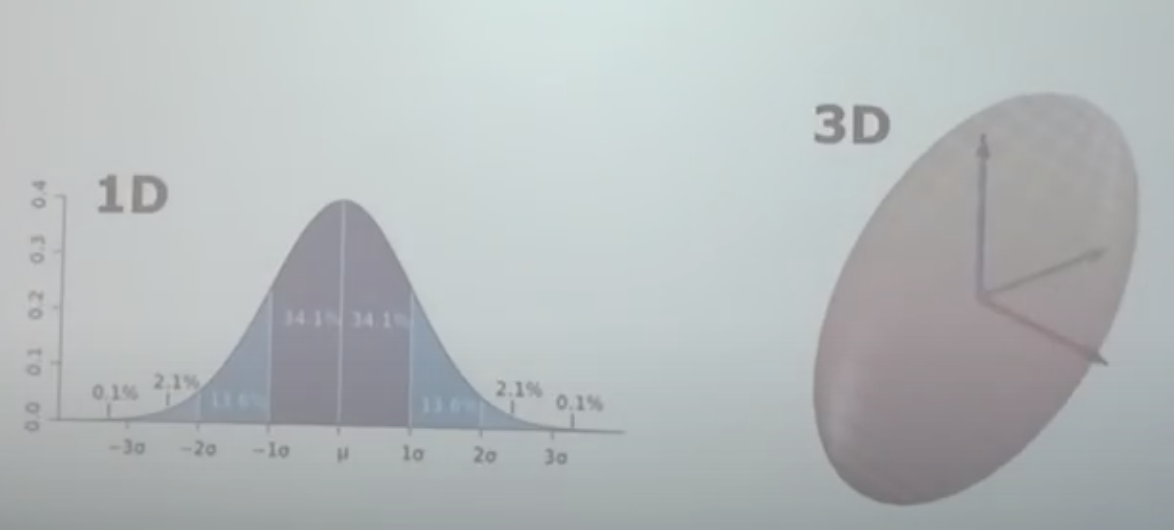
\includegraphics[scale=0.5]{gaussdist}
\end{center}

In the 1D plot, the range on the x-axis from $-3\sigma$ to $3\sigma$ covers approximately $99\%$ of the probability mass, so most events will fall in this area. This distribution can be represented in 2D by an ellipse, and 3D by an ellipsoid.

\textbf{Marginalization and conditioning}

Given
\begin{equation*}
    x = 
    \begin{pmatrix}
         x_a \\ x_b
    \end{pmatrix}
    \qquad
    p(x) = \mathcal{N}
\end{equation*}

The marginals are Gaussians
\begin{equation*}
    p(x_a) = \mathcal{N}
    \qquad
    p(x_b) = \mathcal{N}
\end{equation*}

as well as the conditionals.
\begin{equation*}
    p(x_a | x_b) = \mathcal{N}
    \qquad
    p(x_b | x_a) = \mathcal{N}
\end{equation*}

Here, given that the distribution has two variables: $x_a$ and $x_b$, which both have Gaussian distributions - the corresponding marginal, conditional, as well as convolutional models, then all have Gaussian distributions too.

\textbf{Marginalization}

Given 
\begin{equation*}
    p(x) = p(x_a, x_b) = \mathcal{N}(\mu, \Sigma)
\end{equation*}
\begin{equation*}
    with 
    \qquad
    \mu =
    \begin{pmatrix}
         \mu_a \\ \mu_b
    \end{pmatrix}
    \qquad
    \Sigma = 
    \begin{pmatrix}
         \Sigma_{aa} & \Sigma_{ab} 
         \\ \Sigma_{ba} & \Sigma_{bb}
    \end{pmatrix}
\end{equation*}

The marginal distribution is
\begin{equation*}
    p(x_a) = \int p(x_a, x_b) dx_b = \mathcal{N} (\mu, \Sigma)
\end{equation*}
\begin{equation*}
    with
    \qquad
    \mu = \mu_a
    \qquad
    \Sigma = \Sigma_{aa}
\end{equation*}

This is how to marginalize out a variable - a relatively simple process. So if one has a high-dimensional Gaussian distribution, and wants the marginal for a small number of elements, all that is needed is to cut out the relevant part of the mean vector, and cut out the relevant part of the co-variance matrix.

\textbf{Conditioning}

Given 
\begin{equation*}
    p(x) = p(x_a, x_b) = \mathcal{N}(\mu, \Sigma)
\end{equation*}
\begin{equation*}
    with 
    \qquad
    \mu =
    \begin{pmatrix}
         \mu_a \\ \mu_b
    \end{pmatrix}
    \qquad
    \Sigma = 
    \begin{pmatrix}
         \Sigma_{aa} & \Sigma_{ab} 
         \\ \Sigma_{ba} & \Sigma_{bb}
    \end{pmatrix}
\end{equation*}

The conditional distribution is
\begin{equation*}
    p(x_a | x_b) = \frac{p(x_a, x_b)} {p(x_b)} = \mathcal{N} (\mu, \Sigma)
\end{equation*}
\begin{equation*}
    with
    \qquad
    \mu = \mu_a + \Sigma_{ab} \Sigma_{bb}^{-1} (b - \mu_b)
\end{equation*}
\begin{equation*}
    and
    \qquad
    \Sigma = \Sigma_{aa} - \Sigma_{ab} \Sigma_{bb}^{-1} \Sigma_{ba}
\end{equation*}

The conditional distribution here is normally distributed, but the mean and the co-variance matrix are much harder to calculate. 
The important term to note is the $\Sigma_{bb}^{-1}$. This implies that if one has a high-dimensional Gaussian distribution, and wants to estimate a small quantity out of that, given that the rest is known, it is a very costly operation, because a large part of the original co-variance matrix needs to be operated on.

Also, if one has very little knowledge about the variable $b$, i.e. it has an extremely high uncertainty (and so a very high $\Sigma$), then when inverted the term $\Sigma_{bb}^{-1}$ basically goes to zero. So the derived mean becomes dependent on only $a$.

\subsection{Linear models}

To use the Kalman filter, both the motion and observation models must be linear functions. They are represented as follows.

\begin{equation*}
    x_t = A_t x_{t-1} + B_t u_t + \epsilon_t
\end{equation*}
\begin{equation*}
    z_t = C_t x_t + \delta_t
\end{equation*}

where
\begin{itemize}
    \item $A_t$, $B_t$ and $C_t$ are time-varying matrices
    \item $\epsilon_t$ and $\delta_t$ are noise terms
    \item all remaining variables are the same as usual
\end{itemize}

The presence of the matrices makes both the equations linear (in more than one dimension). For example, the second equation becomes a linear mapping from the world state to the observation state.

The matrix $A$ can be said to represent how the world state changes when no motion command is executed. So typically, it would be the identity matrix (causing no change in the robot's pose if it is at rest). However, in some cases, if an object is already in motion, then $A$ would be different. Similarly, $B$ is a representation of how the physics of the robot's motion affects its world state.

The two equations in a sense are indicative of the mean values for both models; the uncertainty must be taken into account and generated in a later step of the process.

\textbf{Components of a Kalman filter}

\begin{itemize}
    \item $A_t$: an $n$x$n$ matrix that describes how the state evolves from $t-1$ to $t$ without controls or noise.
    \item $B_t$: an $n$x$l$ matrix that describes how the control $u_t$ changes the state from $t-1$ to $t$. Here, $n$ is the dimensionality of the state, and $l$ is the dimensionality of the odometry command. In reality, B should be non-linear (e.g. containing terms of $sin$, $cos$, and the like), but since the requirement of the model is to be linear, it must be made linear in some way.
    \item $C_t$: a $k$x$n$ matrix that describes how to map the state $x_t$ to an observation $z_t$. Here, $k$ is the dimensionality of the observation. In a sense, this matrix defines what one should expect to observe, given that the world is in the current state.
    \item $\epsilon_t$ and $\delta_t$: random variables representing the process and measurement noise that are assumed to be independent and normally distributed, with co-variance matrices $R_t$ and $Q_t$ respectively.
\end{itemize}

Note that if nothing is known about the world, the corresponding Gaussian could be thought of as having a zero mean and a co-variance matrix with close-to-infinity entries - this would represent a kind of uniform distribution.

\textbf{Linear motion model}

Under the Gaussian noise assumption, with the linear requirement, how does the motion model now look?

\begin{equation*}
    p(x_t| u_t, x_{t-1}) = \eta * exp(-\frac{1}{2} * \textbf{?})
\end{equation*}

To deduce the mean of the required Gaussian, consider that one knows the previous state of the system, and which command has just been executed. This allows one to compute for every possible pose, the current state, using the linear model just defined.

\begin{equation*}
    p(x_t| u_t, x_{t-1}) = det(2\pi R_t)^{-\frac{1}{2}} * exp(-\frac{1}{2} * (x_t - A_t x_{t-1} - B_t u_t)^T * R_t^{-1} * (x_t - A_t x_{t-1} - B_t u_t) )
\end{equation*}

where $R_t$ describes the noise of the motion.

\textbf{Linear observation model}

Using a similar approach to derive the Gaussian distribution using the linear approach here,

\begin{equation*}
    p(z_t| x_t) = det(2\pi Q_t)^{-\frac{1}{2}} * exp(-\frac{1}{2} * (z_t - C_t x_t)^T * Q_t^{-1} * (z_t - C_t x_t) )
\end{equation*}

where $Q_t$ describes the measurement noise. Thus, having described both models using Gaussian distributions, one can now plug them into the Kalman filter.

\subsection{Putting the models together}

Given an initial Gaussian belief, the new belief obtained is always Gaussian too. Knowing the truth of this statement, and referring back to the two main steps of the Bayes filter (prediction and correction):

\begin{equation*}
    \overline{bel}(x_t) = \int_{x_{t-1}} \underline{p(x_t | x_{t-1}, u_t)} * \underline{bel(x_{t-1})} dx_{t-1}
\end{equation*}

\begin{equation*}
    bel(x_t) = \eta * \underline{p(z_t | x_t)} * \underline{\overline{bel}(x_t)}
\end{equation*}

Since it is now known how to specify each of the distributions used in these equations, and also that each of them is Gaussian, it is evident that their sum (integral) will be Gaussian as well.

\textbf{Kalman filter algorithm}

\begin{enumerate}
    \item Kalman-filter ($\mu_{t-1}, \Sigma_{t-1}, u_t, z_t$):
    \item \hspace{2em} $\overline{\mu}_t = A_t \mu_{t-1} + B_t \mu_t$
    \item \hspace{2em}  $\overline{\Sigma}_t = A_t \Sigma_{t-1} A_t^T + R_t$
    \item \hspace{2em} $K_t = \overline{\Sigma}_t C_t^T (C_t \overline{\Sigma}_t C_t^T + Q_t) ^{-1}$
    \item \hspace{2em} $\mu_t = \overline{\mu}_t + K_t(z_t - C_t \overline{\mu}_t)$
    \item \hspace{2em} $\Sigma_t = (I - K_t C_t) \overline{\Sigma}_t$
    \item \hspace{2em} return $\mu_t, \Sigma_t$
\end{enumerate}

Lines 2 and 3 are the prediction steps; lines 4 and 6 are the correction steps. The various expressions are derived by replacing the Gaussians produced in the previous section into the two integrals at the beginning of the current section. The overline bar over certain symbols indicates a mean.

In line 3, one sees that the new uncertainty is the old uncertainty plus the uncertainty created by the current motion step. The matrix $A$ is used here partly to scale the system.

Going to the correction step and looking at the original integral expression, it can be seen that two Gaussians are being multiplied in this expression. When two Gaussians are multiplied together, the mean of the new Gaussian produced is the weighted mean of the means of the individual Gaussians, the weights being the uncertainties of the individual Gaussians. Basically, this means that if there is one Gaussian that is very certain and one that is very uncertain, the product of both will be a Gaussian which is very close to the certain distribution.

Moving to the term $K_t$, it is referred to as the Kalman gain. It represents the trade-off between motion uncertainty and observation uncertainty. Looking at some examples to understand this,

\begin{itemize}
    \item Suppose the measurement noise, $Q_t$ is zero. This makes $K_t = C^{-1}$, which when plugged in to the next equations, ultimately leads to $\mu_t$ being dependent fully and only on $z_t$ - that is, the zero uncertainty in the observation model has made the estimated current state completely based on the current observation made.
    \item Conversely, if $Q_t$ tends to infinity, then $K_t$ tends to zero. This ultimately leads to $\mu_t$ having zero dependence on the observation made.
\end{itemize}

\textbf{An example}

\begin{center}
    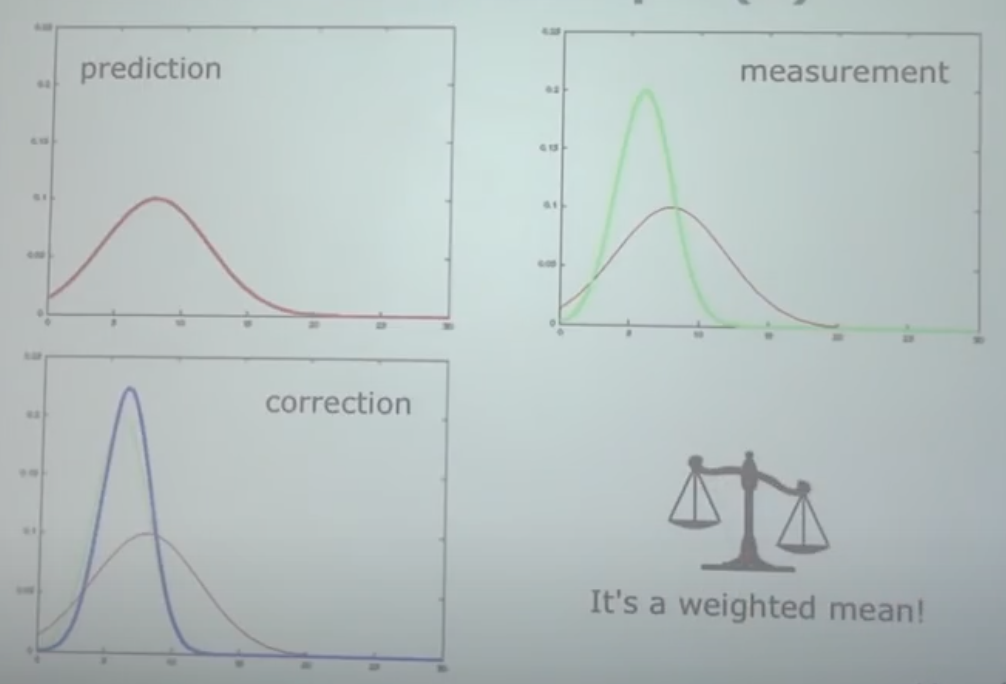
\includegraphics[scale=0.5]{1dkalmeg1}
\end{center}

\begin{itemize}
    \item red curve: prediction distribution
    \item green curve: observation distribution
    \item blue curve: final distribution with correction
\end{itemize}

The corrected curve in this case is closer to the observation/measurement curve in terms of the mean and variance, as the observation has less uncertainty here.

As the robot makes its next movement, the odometry uncertainty will remain the same while the observation uncertainty will increase due to the uncertainty of the previous state. Hence the corrected curve obtained now will have a greater spread (more uncertainty) than the previous corrected curve.

\subsection{Kalman filter assumptions}

What if the system does not follow the assumptions of Gaussian distributions and noise, and linear models, as in reality? Most realistic problems in robotics involve non-linear functions. This would give rise to equations like the following:

\begin{equation*}
    x_t = g(u_t, x_{t-1}) + \epsilon_t
    \qquad
    z_t = h(x_t) + \delta_t
\end{equation*}

where $g$ and $h$ are non-linear functions.

\textbf{The linearity assumption}

An important property that the Kalman filter makes use of, is that a Gaussian distribution, when mapped through a linear function, results in another Gaussian, as shown below.

\begin{center}
    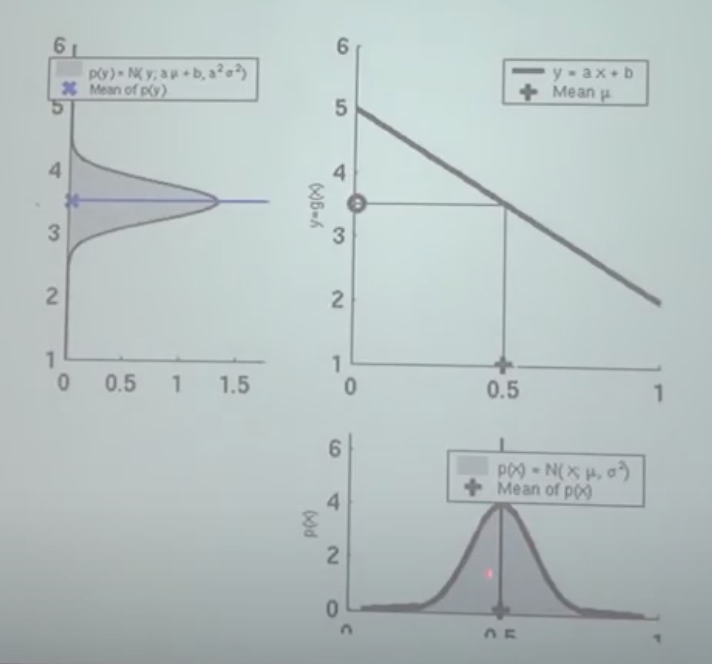
\includegraphics[scale=0.5]{linasm}
\end{center}

However, when one maps it through a non-linear function, a vastly different distribution is obtained:

\begin{center}
    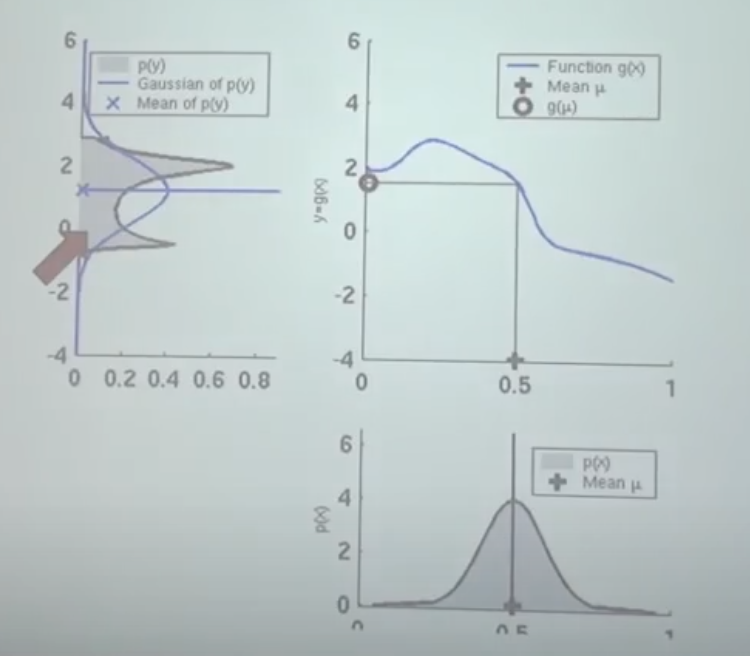
\includegraphics[scale=0.5]{nldist}
\end{center}

Thus the application of the non-linear function in a sense destroys the Gaussian distribution, which the Kalman filter can no longer be applied to. The way to resolve this is to use local linearization, which leads to an extension of the Kalman filter.

The extended Kalman filter fixes this problem of non-linear functions by linearizing those functions, and then proceeding with the steps of the normal filter.

\subsection{EKF linearization: first order Taylor expansion}

Prediction step:

\begin{equation*}
    g(u_t, x_{t-1}) \approx g(u_t, \mu_{t-1}) + \frac {\delta g(u_t, \mu_{t-1})} {\delta x_{t-1}} * (x_{t-1} - \mu_{t-1})
\end{equation*}

Correction step:

\begin{equation*}
    h(x_t) \approx h(\overline{\mu}_t) + \frac {\delta h(\overline{\mu}_t)} {\delta x_t} * (x_t - \overline{\mu}_t)
\end{equation*}

where

\begin{equation*}
    \frac {\delta g(u_t, \mu_{t-1})} {\delta x_{t-1}} =: G_t
    \qquad
    and
    \qquad
    \frac {\delta h(\overline{\mu}_t)} {\delta x_t} =: H_t
\end{equation*}

are Jacobians. A Jacobian matrix is a non-square matrix $mxn$ in general.

Note that given a vector-valued function,

\begin{equation*}
    g(x) = 
    \begin{pmatrix}
    g_1(x) \\ g_2(x) \\ \vdots \\ g_m(x)
    \end{pmatrix}
\end{equation*}

the Jacobian matrix is defined as

\begin{equation*}
    G_x = 
    \begin{pmatrix}
    \frac{\delta g_1}{\delta x_1} & \frac{\delta g_1}{\delta x_2} & \ldots & \frac{\delta g_1}{\delta x_n}
    \\ 
    \frac{\delta g_2}{\delta x_1} & \frac{\delta g_2}{\delta x_2} & \ldots & \frac{\delta g_2}{\delta x_n}
    \\
    \vdots & \vdots & \ldots & \vdots
    \\
    \frac{\delta g_m}{\delta x_1} & \frac{\delta g_m}{\delta x_2} & \ldots & \frac{\delta g_m}{\delta x_n}
    \end{pmatrix}
\end{equation*}

where $m$ is the dimension of the vector function, and $n$ is the number of variables involved. It is a kind of generalization from the 1D derivative, for the higher-dimensional case.

Thus, the Jacobian gives the orientation of the tangent plane to the vector-valued function at a given point. It can also be said to generalize the gradient of a scalar-valued function.

Hence the presence of the Jacobian matrices in the prediction and correction steps linearizes the respective functions - but only at that specific linearization point. So for different linearization points, i.e. different states, the Jacobian will need to be recomputed.

\begin{center}
    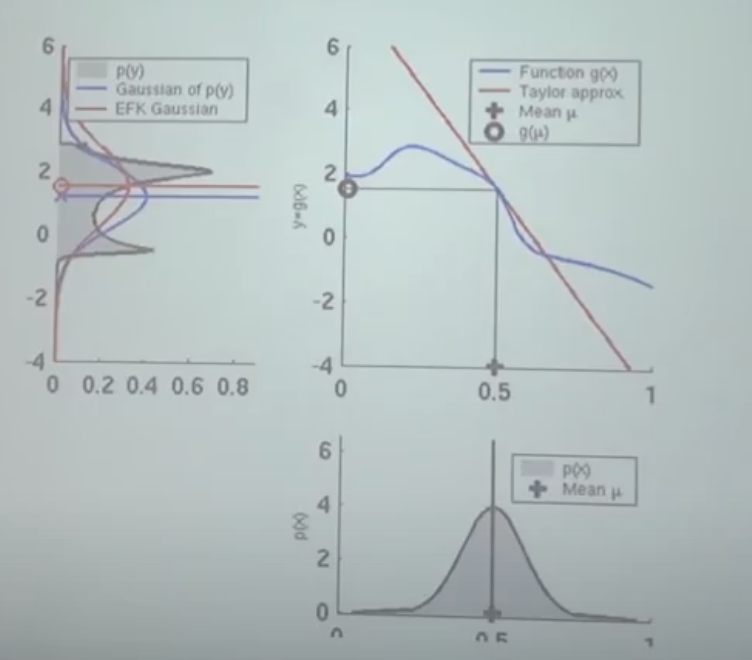
\includegraphics[scale=0.5]{ekfdist}
\end{center}

The resulting curve is thus once again a Gaussian, represented by the red curve in the figure above. Hence, when we linearize the function at a certain point, the less the spread of the initial Gaussian about that point, the less the difference between the initial Gaussian (blue curve in final figure) and the Gaussian produced using the EKF linearization (red curve in final figure), i.e. the better the approximation is.

\textbf{Applying EKF to the models}

Motion model:
\begin{equation*}
    p(x_t| u_t, x_{t-1}) \approx det(2\pi R_t)^{-\frac{1}{2}} * exp(-\frac{1}{2} * (x_t - g(u_t, \mu_{t-1})) - G_t(x_{t-1} - \mu_{t-1})^T 
\end{equation*}
\begin{equation*}
    * R_t^{-1} * (x_t - g(u_t, \mu_{t-1})) - G_t(x_{t-1} - \mu_{t-1}) )
\end{equation*}

Observation model:
\begin{equation*}
    p(z_t| x_t) = det(2\pi Q_t)^{-\frac{1}{2}} * exp(-\frac{1}{2} * (z_t - h(\overline{\mu}_t) - H_t (x_t - \overline{\mu}_t))^T * Q_t^{-1} * (z_t - h(\overline{\mu}_t) - H_t (x_t - \overline{\mu}_t)) )
\end{equation*}

where $R_t$ and $Q_t$ describe the motion noise and measurement noise respectively.

\textbf{Extended Kalman filter algorithm}

\begin{enumerate}
    \item Extended-Kalman-filter ($\mu_{t-1}, \Sigma_{t-1}, u_t, z_t$):
    \item \hspace{2em} $\overline{\mu}_t = g(u_t, \mu_{t-1})$
    \item \hspace{2em} $\overline{\Sigma}_t = G_t \Sigma_{t-1} G_t^T + R_t$
    \item \hspace{2em} $K_t = \overline{\Sigma}_t H_t^T (H_t \overline{\Sigma}_t H_t^T + Q_t) ^{-1}$
    \item \hspace{2em} $\mu_t = \overline{\mu}_t + K_t(z_t - h(\overline{\mu}_t))$
    \item \hspace{2em} $\Sigma_t = (I - K_t H_t) \overline{\Sigma}_t$
    \item \hspace{2em} return $\mu_t, \Sigma_t$
\end{enumerate}

The only differences in this implementation of the Kalman filter are that the original linear functions have been replaced with the derived linearized functions, that is $A_t$ has been replaced with $G_t$, and $C_t$ has been replaced by $H_t$.

So the extended Kalman filter is the same as the standard Kalman filter, except that it uses linear approximations of non-linear functions. Also, $G_t$ and $H_t$ need to be recomputed at every time interval, contrary to $A_t$ and $C_t$ in the standard filter. Also, if $g$ and $h$ turn out to be linear functions, the implementation will give the exact same result as the standard filter does in this case.

The complexity of the filter can be represented as $O(k^{2.4} + n^2)$. The exponent of the first term is derived from the fact that a matrix inversion is required in the observation model, and that of the second term is derived from the fact that $n$x$n$ square matrices are present. Hence, the larger the number of observation parameters, or world-state parameters, the more costly the calculation gets.

\pagebreak


\section{EKF SLAM}

Now, one can start to implement the EKF SLAM method into the localization algorithm of the robot. Here, the map being considered will be in the form of landmark locations - things the robot can identify via its sensor readings or camera images, and calculate the corresponding poses for. 

As usual, the Kalman filter will be used as a solution to the online SLAM problem:
\begin{equation*}
    p(x_t,m|z_{1:t}, u_{1:t})
\end{equation*}

\subsection{State representation}

Beginning with defining the state $\mu$ of the robot (assuming it is in the 2D plane), $\mu$ will be a vector having its first three dimensions $x$, $y$ and $\theta$ describing the pose of the robot, and the remaining dimensions describing the $x$-$y$ coordinates of the landmarks' positions.

\begin{equation*}
    x_t = ( x, y, \theta, \qquad m_{1,x}, m_{1,y}, \ldots m_{n,x}, m_{n,y})^T
\end{equation*}

Thus, a map with $n$ landmarks will give rise to a $3+2n$ dimensional Gaussian distribution.

The belief will then be represented by:
\begin{equation*}
    \begin{pmatrix}
        x \\ y \\ \theta \\ 
        m_{1,x} \\ m_{1,y} \\ \vdots \\
        m_{n,x} \\ m_{n,y}
    \end{pmatrix}
    \begin{pmatrix}
        \sigma_{xx} && \sigma_{xy} && \sigma_{x\theta} && \sigma_{xm_{1,x}} && \sigma_{xm_{1,y}} && \hdots && \sigma_{xm_{n,x}} && \sigma_{xm_{n,y}}
        \\
        \sigma_{yx} && \sigma_{yy} && \sigma_{y\theta} && \sigma_{ym_{1,x}} && \sigma_{ym_{1,y}} && \hdots && \sigma_{ym_{n,x}} && \sigma_{ym_{n,y}}
        \\
        \sigma_{\theta x} && \sigma_{\theta y} && \sigma_{\theta \theta} && \sigma_{\theta m_{1,x}} && \sigma_{\theta m_{1,y}} && \hdots && \sigma_{\theta m_{n,x}} && \sigma_{\theta m_{n,y}}
        \\
        \sigma_{m_{1,x}x} && \sigma_{m_{1,x}y} && \sigma_{\theta} && \sigma_{m_{1,x}m_{1,x}} && \sigma_{m_{1,x}m_{1,y}} && \hdots && \sigma_{m_{1,x}m_{n,x}} && \sigma_{m_{1,x}m_{n,y}}
        \\
        \sigma_{m_{1,y}x} && \sigma_{m_{1,y}y} && \sigma_{\theta} && \sigma_{m_{1,y}m_{1,x}} && \sigma_{m_{1,y}m_{1,y}} && \hdots && \sigma_{m_{1,y}m_{n,x}} && \sigma_{m_{1,y}m_{n,y}}
        \\
        \vdots && \vdots && \vdots && \vdots && \vdots && \ddots && \vdots && \vdots
        \\
        \sigma_{m_{n,x}x} && \sigma_{m_{n,x}y} && \sigma_{\theta} && \sigma_{m_{n,x}m_{1,x}} && \sigma_{m_{n,x}m_{1,y}} && \hdots && \sigma_{m_{n,x}m_{n,x}} && \sigma_{m_{n,x}m_{n,y}}
        \\
        \sigma_{m_{n,y}x} && \sigma_{m_{n,y}y} && \sigma_{\theta} && \sigma_{m_{n,y}m_{1,x}} && \sigma_{m_{n,y}m_{1,y}} && \hdots && \sigma_{m_{n,y}m_{n,x}} && \sigma_{m_{n,y}m_{n,y}}
    \end{pmatrix}
\end{equation*}

where the column vector and the right-hand-side matrix are $\mu$, the pose of the robot, and $\Sigma$ respectively. $\Sigma$ can be considered as having three main sections:

\begin{itemize}
    \item The $3x3$ matrix in the upper left corner which is the co-variance matrix corresponding to the pose of the robot
    \item The $2nx2n$ matrix in the bottom right corner which holds the uncertainties of the landmarks' positions and their correlations
    \item The remaining isolated rectangular matrices which indicate the correlations between the robot's pose and the locations of the landmarks
\end{itemize}

A more compact representation of this belief of state is as follows:

\begin{equation*}
    \begin{pmatrix}
    x_R \\ m_1 \\ \vdots \\ m_n
    \end{pmatrix}
    \begin{pmatrix}
    \Sigma_{x_R x_R} && \Sigma_{x_R m_1} && \hdots && \Sigma_{x_R m_n}
    \\
    \Sigma_{m_1 x_R} && \Sigma_{m_1 m_1} && \hdots && \Sigma_{m_1 m_n}
    \\
    \vdots && \vdots && \ddots && \vdots
    \\
    \Sigma_{m_n x_R} && \Sigma_{m_n m_1} && \hdots && \Sigma_{m_n m_n}
    \end{pmatrix}
\end{equation*}

An even more compact representation could be (note $x_R \rightarrow x$):

\begin{equation*}
    \begin{pmatrix}
    x \\ m
    \end{pmatrix}
    \begin{pmatrix}
    \Sigma_{xx} && \Sigma_{xm}
    \\
    \Sigma_{mx} && \Sigma_{mm}
    \end{pmatrix}
\end{equation*}

\subsection{The filter cycle}

\begin{enumerate}
    \item State prediction: take the control command and estimate the new state of the robot given this command.
    \item Measurement prediction: evaluating the function $h$ at the predicted mean $\mu$ - i.e. what one is expected to observe given the current belief of where the robot is.
    \item Measurement: making observations via sensor input.
    \item Data association: understanding which landmark(s) correspond(s) to what the robot is currently observing, and obtaining the difference between the expected and actual observation.
    \item Update: correcting the belief of state based on the observations.
\end{enumerate}

\subsection{State prediction}

Assuming that the robot does not modify the environment (it only changes its own state, not that of the landmarks), when the robot receives a control command and makes a movement, only $x_R$ (the robot's pose) must be updated.

In the co-variance matrix, the first row and first column of the above representation must be updated. The computational complexity of such an operation is O(n), i.e. linear in n, the number of landmarks. This is quite efficient for such an operation.

Once the control command execution is complete, the robot takes into account the current belief of its state, and computes the predicted measurements for the landmarks around it - it assumes their positions based on its current knowledge of the state.

Next, the real measurements are taken. The robot now must make a data association by deciding which landmark(s) the observation(s) correspond to, and calculate the difference(s) between its estimate and the actual measurement.

Based on this difference, the mean vector for the state can then be updated, leading to the entire co-variance matrix getting updated via the Kalman gain method. The complexity of this computation is O($n^2$). Hence, the sensor observation is much more costly than the initial state updation.

\subsection{A concrete example}

\textbf{Initialization}

The setup for the problem:

\begin{itemize}
    \item Robot moves in the 2D plane (pose described by ($x, y, \theta$)
    \item Velocity-based motion model
    \item Robot observes point landmarks (x,y)
    \item A range-bearing sensor: measures distance and orientation of the landmark with respect to the heading of the robot
    \item Known data associations: whenever one sees a landmark, one knows which landmark it corresponds to in the map
    \item Known number of landmarks
\end{itemize}

\begin{equation*}
    \begin{pmatrix}
    x_R \\ m_1 \\ \vdots \\ m_n
    \end{pmatrix}
    \begin{pmatrix}
    \Sigma_{x_R x_R} && \Sigma_{x_R m_1} && \hdots && \Sigma_{x_R m_n}
    \\
    \Sigma_{m_1 x_R} && \Sigma_{m_1 m_1} && \hdots && \Sigma_{m_1 m_n}
    \\
    \vdots && \vdots && \ddots && \vdots
    \\
    \Sigma_{m_n x_R} && \Sigma_{m_n m_1} && \hdots && \Sigma_{m_n m_n}
    \end{pmatrix}
\end{equation*}

To start off with, the mean vector and co-variance matrix must be initialized. The initial position of the robot can be taken as the origin, in order to define the frame of reference. Hence, we initialize the parameters as such:

\begin{equation*}
    x_R = 
    \begin{pmatrix}
    0 \\ 0 \\ 0
    \end{pmatrix}
    \qquad
    \Sigma_{x_R x_R} = 
    \begin{pmatrix}
    0 && 0 && 0 \\ 0 && 0 && 0 \\ 0 && 0 && 0
    \end{pmatrix}
\end{equation*}

Now since the robot starts in its own reference frame, all the landmarks are unknown. Hence the uncertainty in their positions can be considered to be infinite. So the complete initialization of the belief would be as follows:

\begin{equation*}
    \mu_0 = 
    \begin{pmatrix}
        0 \\ 0 \\ 0 \\ 0 \\ \vdots \\ 0
    \end{pmatrix}
    \qquad
    \Sigma_0 = 
    \begin{pmatrix}
        0 && 0 && 0 && 0 && \hdots && 0
        \\
        0 && 0 && 0 && 0 && \hdots && 0
        \\
        0 && 0 && 0 && 0 && \hdots && 0
        \\
        0 && 0 && 0 && \infty && \hdots && 0
        \\
        \vdots && \vdots && \vdots && \vdots && \ddots && \vdots
        \\
        0 && 0 && 0 && 0 && \hdots && \infty
    \end{pmatrix}
\end{equation*}

Practically, the initial belief should only have three dimensions, that is the ones corresponding to the robot's pose, and the matrix sizes should be updated as and when the robot encounters a new landmark. However, this is algorithmically a lot more complex to implement.

Now, the steps of the EKF algorithm must be followed:

\begin{enumerate}
    \item Extended-Kalman-filter ($\mu_{t-1}, \Sigma_{t-1}, u_t, z_t$):
    \item \hspace{2em} $\overline{\mu}_t = g(u_t, \mu_{t-1}$
    \item \hspace{2em} $\overline{\Sigma}_t = G_t \Sigma_{t-1} G_t^T + R_t$
    \item \hspace{2em} $K_t = \overline{\Sigma}_t H_t^T (H_t \overline{\Sigma}_t H_t^T + Q_t) ^{-1}$
    \item \hspace{2em} $\mu_t = \overline{\mu}_t + K_t(z_t - h(\overline{\mu}_t))$
    \item \hspace{2em} $\Sigma_t = (I - K_t H_t) \overline{\Sigma}_t$
    \item \hspace{2em} return $\mu_t, \Sigma_t$
\end{enumerate}

\textbf{Prediction step (motion)}

Starting with line 2, one sees that the new mean estimate is the output of some function $g$ that takes as input the previous mean and the control command.

Using the velocity based motion model, the goal is to update the state space based on the robot's motion. The robot's new pose can be estimated by:

\begin{equation*}
    \begin{pmatrix}
    x' \\ y' \\ \theta '
    \end{pmatrix}
    =
    \begin{pmatrix}
    x \\ y \\ \theta
    \end{pmatrix}
    +
    \begin{pmatrix}
    - \frac{v_t}{\omega_t} sin\theta + \frac{v_t}{\omega_t} sin (\theta + \omega_t \Delta t)
    \\ \frac{v}{\omega_t} cos\theta - \frac{v}{\omega_t} cos (\theta + \omega_t \Delta t) 
    \\ \omega_t \Delta t
    \end{pmatrix}
\end{equation*}
    
where $\theta + \omega \Delta t$ is the current orientation of the robot. The right hand side of the above matrix equation is the definition of the function $g$, i.e.
    
\begin{equation*}
    g_{x,y,\theta} (u_t, (x, y, \theta)^T)
\end{equation*}
    
Theoretically, $g$ should map the entire $2n+3$ state vector to itself, but here it only considers the robot's pose, i.e. only the first 3 dimensions of the entire state vector. So how does one map the output of $g$ to the $2n+3$ dimensional space then? This can be done by modifying the equation as shown:

\begin{equation*}
    \begin{pmatrix}
    x' \\ y' \\ \theta ' \\ \vdots
    \end{pmatrix}
    =
    \begin{pmatrix}
    x \\ y \\ \theta \\ \vdots
    \end{pmatrix}
    +
    F_x^T
    \begin{pmatrix}
    - \frac{v_t}{\omega_t} sin\theta + \frac{v_t}{\omega_t} sin (\theta + \omega_t \Delta t)
    \\ \frac{v}{\omega_t} cos\theta - \frac{v}{\omega_t} cos (\theta + \omega_t \Delta t) 
    \\ \omega_t \Delta t
    \end{pmatrix}
\end{equation*}

where $F_x$ is the $3$ x $(2n+3)$ matrix

\begin{equation*}
    \begin{pmatrix}
        1 && 0 && 0 && 0 && \hdots && 0
        \\
        0 && 1 && 0 && 0 && \hdots && 0
        \\
        0 && 0 && 1 && 0 && \hdots && 0
    \end{pmatrix}
\end{equation*}

\textbf{Updating co-variance}

Now one moves to the third line of the algorithm, for which $G$, the Jacobian of $g$ needs to be computed. (As seen, $R_t$ is the uncertainty of the motion model, which is assumed to be given.)

It is known that $g$ only affects the position of the robot and not the landmarks. Since the position of the landmarks are not changing in the update step, the portion of $G_t$ that represents them will be a $2n$ x $2n$ identity matrix.

\begin{equation*}
    G_t = 
    \begin{pmatrix}
    G_t^x && 0 \\ 0 && I
    \end{pmatrix}
\end{equation*}

where $G_t^x$ is the $3$x$3$ Jacobian of the motion, and I is the $2n$ x $2n$ identity matrix.

To find $G_t^x$, one needs to derive the non-linear function which maps the odometry information to the state update.

\begin{equation*}
    G_t^x = \frac{\partial}{\partial (x, y, \theta)^T}
    \begin{bmatrix}
        \begin{pmatrix}
            x \\ y \\ \theta
        \end{pmatrix}
        +
        \begin{pmatrix}
            - \frac{v_t}{\omega_t} sin\theta + \frac{v_t}{\omega_t} sin (\theta + \omega_t \Delta t)
            \\ \frac{v}{\omega_t} cos\theta - \frac{v}{\omega_t} cos (\theta + \omega_t \Delta t) 
            \\ \omega_t \Delta t
        \end{pmatrix}
    \end{bmatrix}
\end{equation*}

\begin{equation*}
    = I + \frac{\partial}{\partial (x, y, \theta)^T}
    \begin{pmatrix}
        - \frac{v_t}{\omega_t} sin\theta + \frac{v_t}{\omega_t} sin (\theta + \omega_t \Delta t)
        \\ \frac{v}{\omega_t} cos\theta - \frac{v}{\omega_t} cos (\theta + \omega_t \Delta t) 
        \\ \omega_t \Delta t
    \end{pmatrix}
\end{equation*}

The remaining matrix has no dependencies on x and y, so the first two columns of the resulting derivative matrix will be zero.

\begin{equation*}
    = I + 
    \begin{pmatrix}
        0 && 0 && - \frac{v_t}{\omega_t} cos\theta + \frac{v_t}{\omega_t} cos (\theta + \omega_t \Delta t)
        \\ 
        0 && 0 && - \frac{v}{\omega_t} sin\theta + \frac{v}{\omega_t} sin (\theta + \omega_t \Delta t) 
        \\ 
        0 && 0 && 0
    \end{pmatrix}
\end{equation*}

\begin{equation*}
=
\begin{pmatrix}
        1 && 0 && - \frac{v_t}{\omega_t} cos\theta + \frac{v_t}{\omega_t} cos (\theta + \omega_t \Delta t)
        \\ 
        0 && 1 && - \frac{v}{\omega_t} sin\theta + \frac{v}{\omega_t} sin (\theta + \omega_t \Delta t) 
        \\ 
        0 && 0 && 1
    \end{pmatrix}
\end{equation*}

Looking at the $G_t$ matrix as a whole now, it is clear that it is simply an identity matrix with two additional non-zero elements in the third column. 

The presence of these two elements linearizes the dependencies on sin and cosine of the function. For linear movement these two would hence be zero.

Now that all the required quantities are known, the third step of the algorithm can be carried out in full:

\begin{equation*}
    \overline{\Sigma}_t 
    \qquad 
    = 
    \qquad
    G_t \Sigma_{t-1} G_t^T + R_t
\end{equation*}

\begin{equation*}
    = 
    \begin{pmatrix}
            G_t^x && 0 \\ 0 && I
    \end{pmatrix}
    \begin{pmatrix}
            \Sigma_{xx} && \Sigma_{xm}
            \\
            \Sigma_{mx} && \Sigma_{mm}
    \end{pmatrix}
    \begin{pmatrix}
        (G_t^x)^T && 0 \\ 0 && I    
    \end{pmatrix}
     + R_t
\end{equation*}

\begin{equation*}
    = 
    \begin{pmatrix}
        G_t^x \Sigma_{xx} (G_t^x)^T && G_t^x \Sigma_{xm}
        \\
        (G_t^x \Sigma_{xm})^T && \Sigma_{mm}    
    \end{pmatrix}
     + R_t
\end{equation*}

This form of the equation now perfectly shows exactly which parts of the co-variance matrix get updated via $G_t^x$.

\textbf{Summarising the prediction step}

\begin{equation*}
    F_x = 
    \begin{pmatrix}
        1 && 0 && 0 && 0 && \hdots && 0
        \\
        0 && 1 && 0 && 0 && \hdots && 0
        \\
        0 && 0 && 1 && 0 && \hdots && 0
    \end{pmatrix}
\end{equation*}

The matrix which maps from the low dimensional to the high dimensional space is defined.

\begin{equation*}
    \overline{\mu}_t = \mu_{t-1} + F_x^T 
    \begin{pmatrix}
    - \frac{v_t}{\omega_t} sin\theta + \frac{v_t}{\omega_t} sin (\theta + \omega_t \Delta t)
    \\ \frac{v}{\omega_t} cos\theta - \frac{v}{\omega_t} cos (\theta + \omega_t \Delta t) 
    \\ \omega_t \Delta t
    \end{pmatrix}
\end{equation*}

The predicted mean is updated via the non-linear function which updates the state based on translational and rotational velocities.

\begin{equation*}
    G_t = I + F_x^T 
    \begin{pmatrix}
        0 && 0 && - \frac{v_t}{\omega_t} cos\theta + \frac{v_t}{\omega_t} cos (\theta + \omega_t \Delta t)
        \\ 
        0 && 0 && - \frac{v}{\omega_t} sin\theta + \frac{v}{\omega_t} sin (\theta + \omega_t \Delta t) 
        \\ 
        0 && 0 && 0
    \end{pmatrix} 
    F_x
\end{equation*}

The Jacobian $G$ of the non-linear function $g$ is computed.

\begin{equation*}
    \overline{\Sigma}_t = G_t \Sigma_{t-1} G_t^T + F_x^T R_t^x F_x
\end{equation*}

The change in the robot's pose does not affect the uncertainty in the landmark's positions, hence $R_t$ is simply mapped back to the high-dimensional space via $F_x$ at this point.

\textbf{The correction step}

To carry out this step, one would proceed along the following lines making the given assumptions:

\begin{itemize}
    \item Data associations are known
    \item $c_t^i = j$: the $i$th measurement taken at time t observes the landmark with index $j$
    \item The landmark is initialized if previously unobserved
    \item The expected observation is computed
    \item The Jacobian of the measurement function $h$ is computed
    \item The remaining process is completed with computation and application of the Kalman gain
\end{itemize}

Often, for data association, the nearest neighbour method is used - the algorithm tries to identify which landmark is the best fit for the observation it has just made, and if it cannot make such a connection, then the observation is, in a sense, discarded.

\textbf{Range-bearing observations}

A range-bearing observation takes the form of 
\begin{equation*}
    z_t^i = (r_t^i, \phi_t^i)^T
\end{equation*}

If a landmark has not been observed, it's coordinates in the state get updated as shown:

\begin{equation*}
    \begin{pmatrix}
        \overline{\mu}_{j,x} \\ \overline{\mu}_{j,y}
    \end{pmatrix}
    =
    \begin{pmatrix}
            \overline{\mu}_{t,x} \\ \overline{\mu}_{t,y}
    \end{pmatrix} 
    + 
    \begin{pmatrix}
            r_t^i cos(\phi_t^i + \overline{\mu}_{t,\theta}
            \\
            r_t^i sin(\phi_t^i + \overline{\mu}_{t,\theta}
    \end{pmatrix}
\end{equation*}

i.e. observed location of landmark j = estimated robot's location + relative measurement. Hence, via this calculation, the position of the landmark is obtained, using the assumptions that the measurement made by the sensors is correct and that the robot is at the right position while making the measurement.

\textbf{The expected observation}

Next, the expected observation of the landmark(s) must be updated based on the current estimate of the state.

\begin{equation*}
    \delta = 
    \begin{pmatrix}
            \delta_x \\ \delta_y
    \end{pmatrix} 
    = 
    \begin{pmatrix}
        \overline{\mu}_{j,x} - \overline{\mu}_{t,x}
        \\
        \overline{\mu}_{j,y} - \overline{\mu}_{t,y}
    \end{pmatrix}
\end{equation*}

Here, $\delta_x$ and $delta_y$ represent the difference in the x and y coordinates between the position of the robot and the position of the landmark.

\begin{equation*}
    q = \delta^T \delta
\end{equation*}

So q represents the square of the Euclidean distance between the robot and the landmark.

\begin{equation*}
    \hat{z}_t^i = 
    \begin{pmatrix}
            \sqrt{q} \\ atan2(\delta_y, \delta_x) - \overline{\mu}_{t, \theta}
    \end{pmatrix} 
    = 
    h(\overline{\mu}_t)
\end{equation*}

These quantities are then used to compute the tuple of distance and orientation that represents the predicted observation. Thus, $h$ is obtained, the function that maps the current state to this observation.

\textbf{Jacobian for the observation}

The $H_t^i$ of the low dimensional state space will first be computed. This is done due to the same principle as the previous Jacobian - all the remaining parts of the high dimensional matrix at this stage will be unchanged and hence their derivative will anyway be zero.

\begin{equation*}
    low H_t^i = 
    \frac{\partial h (\overline{\mu}_t)} {\partial \overline{\mu}_t}
\end{equation*}

This low dimensional H will be a five-element vector: ($x, y, \theta, m_{j,x}, m_{j,y}$). The two additional elements over the pose of the robot correspond to the coordinates of the landmark being observed.

\begin{equation*}
    low H_t^i = 
    \begin{pmatrix}
        \frac {\partial \sqrt{q}} {\partial x} && \frac {\partial \sqrt{q}} {\partial y} && \hdots
        \\
        \frac {\partial atan2(\ldots)} {\partial x} && \frac {\partial atan2(\ldots)} {\partial y} && \hdots
    \end{pmatrix}
\end{equation*}

Looking more closely at how to compute the first element of this matrix:

\begin{equation*}
    \frac {\partial \sqrt{q}} {\partial x} = \frac {1}{2} \frac {1} {\sqrt{q}} 2 \delta_x (-1)
\end{equation*}

\begin{equation*}
    = \frac{1}{q} (- \sqrt{q} \delta_x)
\end{equation*}

Performing similar computations for all the elements of the matrix, one obtains

\begin{equation*}
    low H_t^i = 
    \frac{\partial h (\overline{\mu}_t)} {\partial \overline{\mu}_t}
\end{equation*}

\begin{equation*}
    = \frac{1}{q} 
    \begin{pmatrix}
        -\sqrt{q} \delta_x && -\sqrt{q} \delta_y && 0 && +\sqrt{q} \delta_x && +\sqrt{q} \delta_y
        \\
        \delta_y && -\delta_x && -q && -\delta_y && \delta_x
    \end{pmatrix}
\end{equation*}

This low dimensional $H$ now once again needs to be mapped back to the high dimensional space, with the help of another mapping function $F_{x,j}$:

\begin{equation*}
    F_{x,j} = 
    \begin{pmatrix}
        1 && 0 && 0 && 0 && \hdots && 0 && 0 && 0 && 0 && \hdots && 0
        \\
        0 && 1 && 0 && 0 && \hdots && 0 && 0 && 0 && 0 && \hdots && 0
        \\
        0 && 0 && 1 && 0 && \hdots && 0 && 0 && 0 && 0 && \hdots && 0
        \\
        0 && 0 && 0 && 0 && \hdots && 0 && 1 && 0 && 0 && \hdots && 0
        \\
        0 && 0 && 0 && 0 && \hdots && 0 && 0 && 1 && 0 && \hdots && 0
    \end{pmatrix}
\end{equation*}

where the first section of zeros has $2j-2$ columns, and the second section has $2n-2j$ columns (i.e. the pair of 1s in the middle corresponds to the landmark's coordinates). So finally,

\begin{equation*}
    H_t^i = low H_t^i * F_{x,j}
\end{equation*}

\textbf{Summarising the correction steps}

Now that $H$ has been well defined, one can proceed with the next steps of the algorithm. $Q_t$, the sensor noise term, is something which depends on the specification of the sensor (not taken into account here yet).

Using all the quantities now known, the Kalman gain can be computed easily, and the remaining steps completed. Thus, to summarise the correction process:

\begin{equation*}
    Q_t = 
    \begin{pmatrix}
            \sigma_r^2 && 0 \\ 0 && \sigma_{\phi}^2
    \end{pmatrix}
\end{equation*}

For all observed features $z_t^i = (r_t^i, \phi_t^i)^T$ do
\begin{itemize}
    \item $j = c_t^i$
    \item if landmark j is never seen before:
    \begin{equation*}
    \begin{pmatrix}
        \overline{\mu}_{j,x} \\ \overline{\mu}_{j,y}
    \end{pmatrix}
    =
    \begin{pmatrix}
            \overline{\mu}_{t,x} \\ \overline{\mu}_{t,y}
    \end{pmatrix} 
    + 
    \begin{pmatrix}
            r_t^i cos(\phi_t^i + \overline{\mu}_{t,\theta}
            \\
            r_t^i sin(\phi_t^i + \overline{\mu}_{t,\theta}
    \end{pmatrix}
    \end{equation*}
    \item endif
    \item \begin{equation*}
            \delta = 
        \begin{pmatrix}
                \delta_x \\ \delta_y
        \end{pmatrix} 
        = 
        \begin{pmatrix}
            \overline{\mu}_{j,x} - \overline{\mu}_{t,x}
            \\
            \overline{\mu}_{j,y} - \overline{\mu}_{t,y}
        \end{pmatrix}
        \end{equation*}
        \item $q = \delta^T \delta$
        \item \begin{equation*}
        \hat{z}_t^i = 
        \begin{pmatrix}
                \sqrt{q} \\ atan2(\delta_y, \delta_x) - \overline{\mu}_{t, \theta}
        \end{pmatrix} 
        = 
        h(\overline{\mu}_t)
    \end{equation*}
    \item \begin{equation*}
        H_t^i = \frac{1}{q} 
        \begin{pmatrix}
            -\sqrt{q} \delta_x && -\sqrt{q} \delta_y && 0 && +\sqrt{q} \delta_x && +\sqrt{q} \delta_y
            \\
            \delta_y && -\delta_x && -q && -\delta_y && \delta_x
        \end{pmatrix}
         * F_{x,j}
    \end{equation*}
    \item Kalman gain, $\overline{\mu}_t$ and $\overline{\Sigma}_t$ are computed
\end{itemize}

endfor

$\mu_t = \overline{\mu}_t$

$\Sigma_t = \overline{\Sigma}_t$

return $\mu_t$, $\Sigma_t$

\textbf{Implementation notes}

\begin{itemize}
    \item The measurement update in a single step requires only one full belief matrix update (and one partial). The landmark information can also be updated simultaneously - it need not be iterated over - however, this is not optimal.
    \item Always normalize the angular components (be wary of the wraparound).
\end{itemize}

\subsection{Loop closure}

After a long traversal through an unknown environment, a robot may come back to a certain point that it had visited before. The ability to recognize and register that it has been at this place before is known as loop closure.

This process mainly involves data association, and may involve high uncertainties. There is a possibility that it is simply visiting a symmetric area of the environment, and this can cause ambiguities. Hence loop closure is a non-trivial decision.

However, the uncertainties tend to collapse after a loop closure (whether the closure was correct or not). This is because the motion uncertainty of the robot increases as it moves through the environment for a greater time. So coming back to a location visited long ago, and recognizing it as already visited, allows the smaller motion uncertainty of that previous time to propagate through the algorithm and reduce all the following uncertainties.

Thus, loop closing reduces the uncertainty in the robot and landmark estimates. This can be exploited when exploring an environment for the sake of better and more accurate maps.

However, wrong loop closures lead to filter divergence, due to the entirely wrong mean estimates and uncertainty estimates that are produced on such a decision.

\end{document}